%\chapter{Cap\'{\i}tulo 1}
%Los cap\'{\i}tulos son las principales divisiones del documento. En estos, se desarrolla el tema del documento. Cada cap\'{\i}tulo debe corresponder a uno de los temas o aspectos tratados en el documento y por tanto debe llevar un t\'{\i}tulo que indique el contenido del cap\'{\i}tulo.\\
%
%Los t\'{\i}tulos de los cap\'{\i}tulos deben ser concertados entre el alumno y el director de la tesis  o trabajo de investigaci\'{o}n, teniendo en cuenta los lineamientos que cada unidad acad\'{e}mica brinda. As\'{\i} por ejemplo, en algunas facultades se especifica que cada cap\'{\i}tulo debe corresponder a un art\'{\i}culo cient\'{\i}fico, de tal manera que se pueda publicar posteriormente en una revista.\\
%
%\section{Subt\'{\i}tulos nivel 2}
%Toda divisi\'{o}n o cap\'{\i}tulo, a su vez, puede subdividirse en otros niveles y s\'{o}lo se enumera hasta el tercer nivel. Los t\'{\i}tulos de segundo nivel se escriben con min\'{u}scula al margen izquierdo y sin punto final, est\'{a}n separados del texto o contenido por un interlineado posterior de 10 puntos y anterior de 20 puntos (tal y como se presenta en la plantilla).\\
%
%\subsection{Subt\'{\i}tulos nivel 3}
%De la cuarta subdivisi\'{o}n en adelante, cada nueva divisi\'{o}n o \'{\i}tem puede ser se\~{n}alada con vi\~{n}etas, conservando el mismo estilo de \'{e}sta, a lo largo de todo el documento.\\
%
%Las subdivisiones, las vi\~{n}etas y sus textos acompa\~{n}antes deben presentarse sin sangr\'{\i}a y justificados.\\
%
%\begin{itemize}
%\item En caso que sea necesario utilizar vi\~{n}etas, use este formato (vi\~{n}etas cuadradas).
%\end{itemize}

\chapter{Marco teórico}\label{cap:Marco}
%
%\section{Black Oil Model}

\section{El medio poroso}\label{sec:porousmedium}

La física en que se apoya la simulación de yacimientos de petróleo incluye el concepto de medio poroso. Un medio poroso se puede entender como un dominio espacial que ocupa parcialmente un sólido y una porción que ocupan los fluidos, a la que se le llama espacio vacío o poroso. Un yacimiento es un medio poroso que ocurre naturalmente, una formación geológica del subsuelo, que, a nivel microscópico, se compone por una red de poros que se pueden interconectar y que permiten almacenar fluidos \citep{Bear2018}.\\

La definición de medio poroso se extiende de la definición de un medio continuo. Un medio continuo, es aquel que no pierde sus propiedades cuando se divide infinitamente, es decir, sus propiedades son continuas en todo punto. Sin embargo, esta definición depende del nivel de observación. A nivel microscópico, si se toman medidas de espacio poroso en diferentes puntos, es posible encontrar unas zonas vacías y otras ocupadas por la roca. Por otro lado, al incrementar el tamaño de la muestra para la medida, es posible notar que las medidas toman valores menos oscilatorios, tal como se muestra en la Figura \ref{fig:medioporoso}. El mínimo tamaño de muestra al que el espacio poroso empieza a tomar un valor constante se le llama volumen de elemento representativo (REV, \cite{Bear2018}). El espacio poroso medido en un REV se denota porosidad ($\phi$), que corresponde a la capacidad de almacenamiento de fluidos a nivel macroscópico.\\

\begin{figure}[h]
	\centering%
	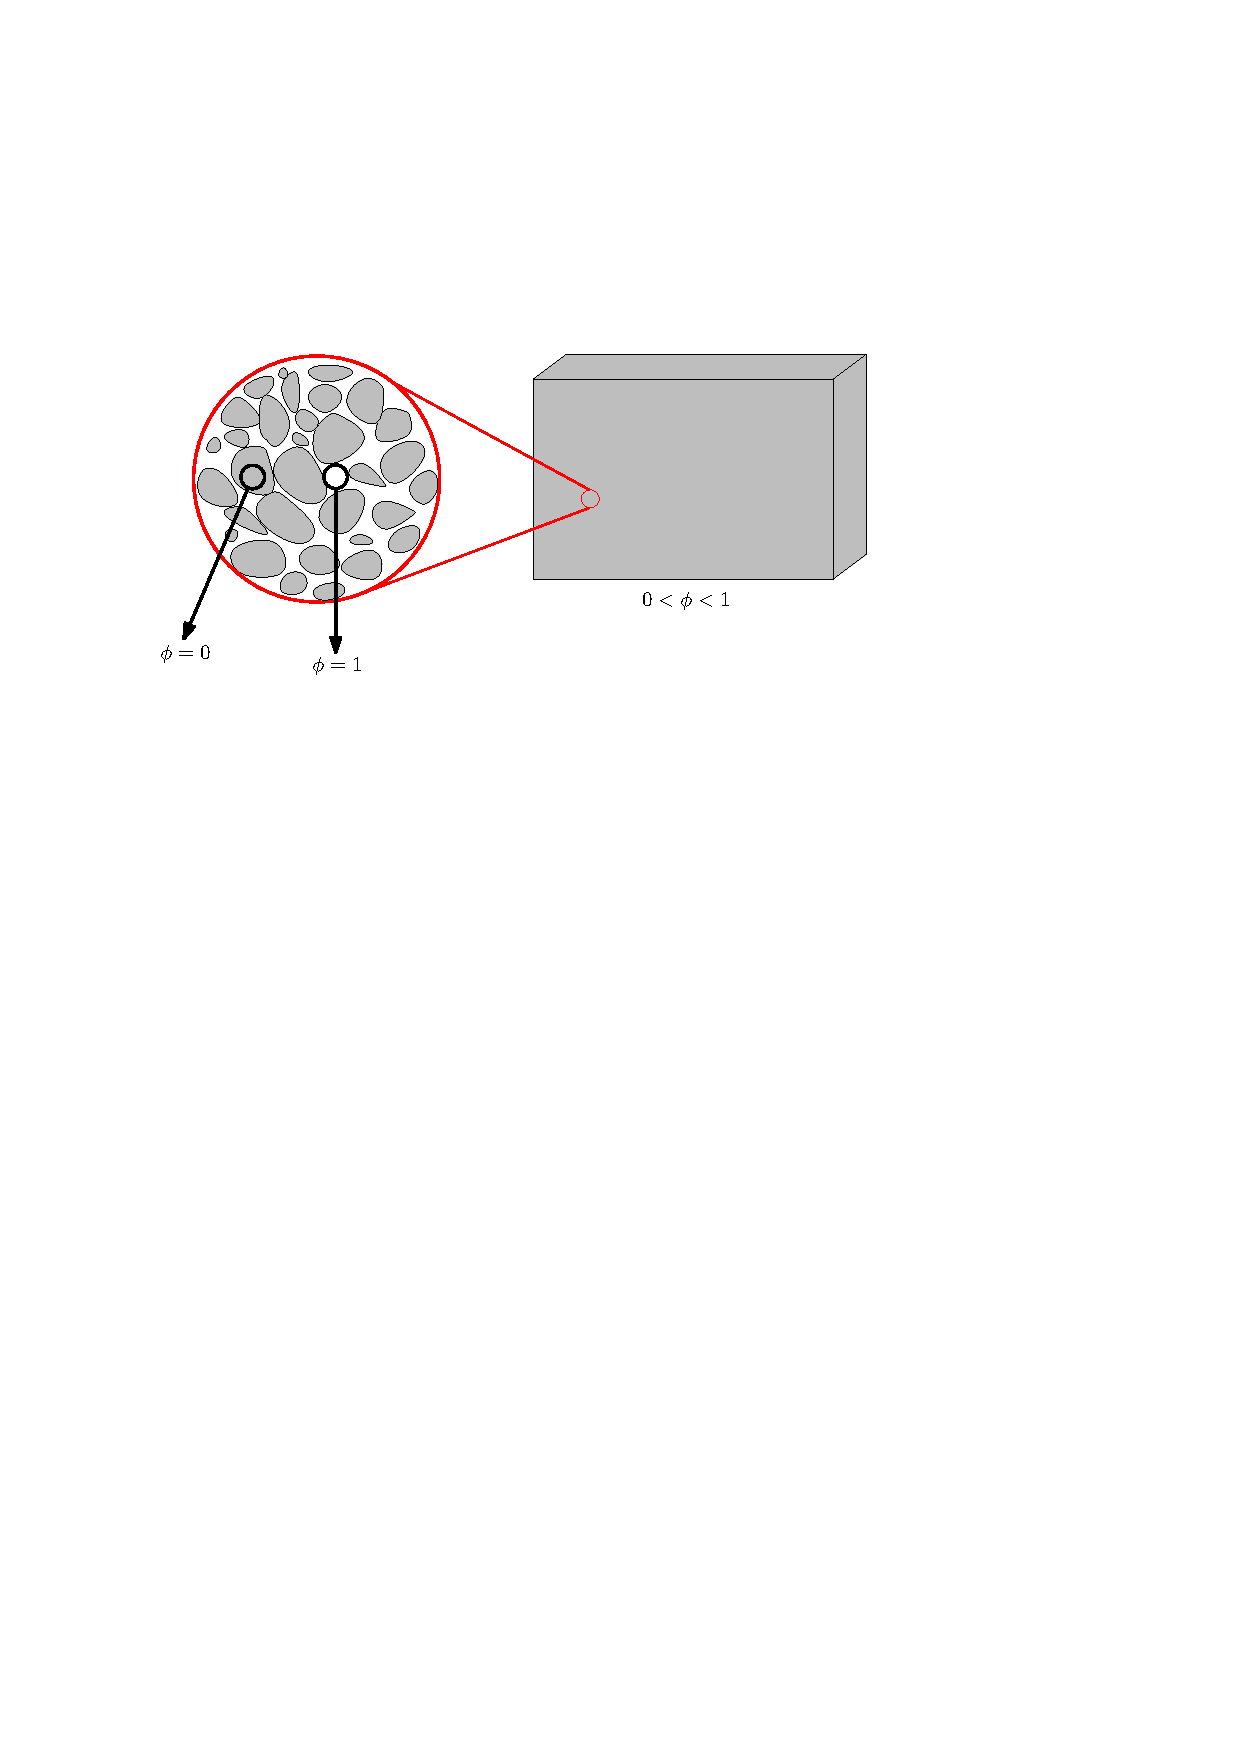
\includegraphics[scale=0.8]{Fig/porous_media.pdf}%
	\caption[Medio poroso y volumen de elemento representativo.]{Medio poroso y volumen de elemento representativo. Elaboración a partir de \cite{Bear2018}.} \label{fig:medioporoso}
\end{figure}
%Adicionalmente, existen gargantas de poro que conectan los poros de la roca, estas gargantas de poro indican la capacidad de la roca de permitir el transporte de los fluidos que puedan existir. La propiedad macroscópica que describe de la capacidad de transportar fluido es la permeabilidad absoluta. La permeabilidad absoluta es una propiedad direccional, es decir que puede variar según la dirección en la que se mida, si la permeabilidad varía su dirección en función del espacio, se dice que el medio es anisotrópico.

\section{Transporte de fluidos en medios porosos}\label{sec:Darcy}

Los fluidos que se almacenan en un yacimiento, en general, se encuentran en un estado estable, el cual se afecta con la aplicación de diferentes campos actuando sobre el dominio físico (el medio poroso). Así, los fluidos se pueden desplazar debido a efectos gravitacionales, cambios de presión y saturación o capilaridad, entre otros.\\ %En esta tesis de maestría se estudia el flujo o transporte dominado por la advección, es decir, el flujo que se da principalmente por gradientes de presión.

El flujo macroscópico de los fluidos se rige por la ley de conservación de momentum en medios porosos o ley de Darcy que se enuncia en la ecuación \ref{ec:DarcyMonofasico}. En esta ley se establece que la velocidad Darcy ($\vec{u}$) de un fluido es proporcional a los gradientes de presión y gravitacionales ($\nabla{\Phi}$ con $\Phi = p + \rho g z$) de un fluido, e inversamente proporcional a su viscosidad ($\mu$). Además, depende de la conductividad del medio poroso, a la cual se le denomina permeabilidad absoluta ($\mathbb{K}$) \citep{Whitaker1986, FANCHI2002108}.
\begin{align}
	\label{ec:DarcyMonofasico} & \vec{u}=\frac{\mathbb{K}}{\mu } \left(\nabla{\Phi}\right)	
\end{align}

%con $\nabla{\Phi_{f}} = \nabla{p} - \rho g \nabla{z}$ 

donde $\mathbb{K}(\vec{x},t)$ es una propiedad direccional con $\vec{x}=(x,y,z)$:
 
\begin{align}
	\mathbb{K} = \left(\begin{array}{ccc}k_{xx}& & \\
	& k_{yy} & \\
	& & k_{zz}
	\end{array}\right)
\end{align}

Estas ecuaciones se aplican para un solo fluido. En el caso de múltiples fluidos ocupando el espacio poroso se usa la ecuación \ref{ec:DarcyMultifasico}, en la cual, se introduce un término de permeabilidad relativa ($kr_{f}(S_{f})$), que depende de la fracción del volumen poroso que ocupa un fluido, la cual se denomina saturación ($S_{f}$).

\begin{align}
\label{ec:DarcyMultifasico} & \vec{u_{f}}=\frac{\mathbb{K}kr_{f}}{\mu_{f} } \nabla{\Phi_{f}}
\end{align}

\subsection{Mojabilidad}\label{subsec:Wettability}
En la mojabilidad se mide la preferencia de la superficie de una roca cuando se moja por determinado fluido o por una combinación de fluidos (mojabilidad intermedia) \citep{chen2007reservoir}. El fluido de preferencia o ``fluido mojante'' se atrapa en los poros más pequeños de la roca, generando una capa del fluido sobre la superficie de la misma \citep{chen2007reservoir}. A la fracción del fluido que se queda atrapado en la roca se le denomina ``saturación irreducible'' ($S_{fc}$) \citep{chen2007reservoir}. \\

\subsection{Presión Capilar}\label{subsec:Capillary}
Cuando existe flujo de dos fluidos, se genera una discontinuidad en la presión de ambos, la cuál se denomina ``presión capilar''. Ésta se calcula como la resta de la presión del ``fluido no mojante'' con la del ``fluido mojante''\citep{chen2007reservoir, FANCHI2002108}. En la Ecuación \ref{ec:presioncapilar} se presenta el cálculo de la ``presión capilar''.
\begin{align}
	\label{ec:presioncapilar}&p_c = p_{\text{fluido no mojante}} - p_{\text{fluido mojante}}
\end{align}

La presión capilar es función de la saturación de uno de los fluidos que se relaciona, según el caso: $p_c(S_{f})$. En el caso de un sistema de tres fluidos, se requieren dos presiones capilares \citep{chen2007reservoir}.

\subsection{Permeabilidad Relativa}\label{subsec:Krs}
La permeabilidad relativa ($k_{r}$) es una relación o fracción de movimiento de un fluido respecto a otro u otros \citep{chen2007reservoir}. Cuando sólo existen dos fluidos, la permeabilidad relativa es función directa de la saturación del fluido correspondiente ($k_{rf}(S_{f})$). Sin embargo, cuando hay tres o más fluidos, ésta puede depender de otras saturaciones ($k_{rf}(S_{f}, ...)$) \citep{chen2007reservoir}.

Cuando existen tres fluidos en un yacimiento de petróleo, obtener información experimental que relacione la permeabilidad relativa conjunta es difícil. En práctica, lo que se hace es medir permeabilidades relativas entre dos fluidos, es decir, los ``contactos'', e interpolar la permeabilidad del fluido de mojabilidad intermedia entre ellas. \citep{Zuo2014}.\\

Existen múltiples métodos de interpolación para obtener la permeabilidad relativa del fluido con más de un contacto \citep{Delshad1989, Blunt2000, Zuo2014}. Para el desarrollo de esta Tesis de Maestría se usa la interpolación de \cite{Baker1988}, la cuál se muestra en la Ecuación \ref{ec:Baker}.

\begin{align}
	\label{ec:Baker}&k_{ro}(S_{g}, S_{w}) = \frac{\left(S_{w}-S_{wc}\right)k_{row} + \left(S_{g}-S_{gc}\right)k_{rgo}}{\left(S_{w}-S_{wc}\right) + \left(S_{g}-S_{gc}\right)}
\end{align}\\

En un sistema de agua, gas y petróleo, se obtiene la permeabilidad relativa del petróleo al agua $k_{row}(S_{w})$ y la permeabilidad relativa del petróleo al gas $k_{rgo}(S_{g})$ y se pondera la permeabilidad relativa del petróleo por la saturación del gas y del agua \citep{Baker1988}.

\section{Simulación de Yacimientos de Petróleo}\label{sec:Simulation}
El dominio de la simulación de yacimientos de petróleo se enmarca dentro del contexto del desarrollo de software científico referido a procesos industriales y de investigación de nuevas tecnologías \citep{Kelly2015}; los cuales requieren la implementación de modelos matemáticos complejos que representan múltiples fenómenos físicos y químicos entre los fluidos. La simulación de yacimientos de petróleo se rige por las leyes de conservación de la masa y del momentum. En estas leyes se describe la acumulación, transporte, fuentes y sumideros de los fluidos como un sistema de ecuaciones diferenciales parciales acopladas para un dominio físico. La solución analítica de estos sistemas, cuando es viable, requiere condiciones que se alejan de los problemas reales \citep{ertekin2001basic}. Por ello, es necesario una solución numérica o simulación. Un modelo de simulación que se usa en la industria es el \textit{Black Oil Model}.%, este hace una simplificación de la composición de los hidrocarburos existentes. Solucionar tales ecuaciones requiere discretizar el tiempo y el dominio físico; usar métodos de solución de sistemas no lineales, y métodos de solución de sistemas lineales así como el precondicionamiento de los mismos. \\ %Estas elecciones tienen un impacto en las capacidades de solución de ecuaciones que surgen de los diferentes problemas físicos.\\
%Más aún, los resultados de la simulación deben ser contrastados con datos experimentales para verificar su concordancia con el fenómeno físico que modelan.\\


\subsection[Modelo \emph{Black Oil} Extendido]{Modelo {\normalfont \bfseries \itshape Black Oil} Extendido}\label{subsec:BOM}

El \textit{Black Oil Model} (BOM) es un modelo de conservación de volumen a condiciones estándar, en el cual, se considera la existencia de tres fluidos en el medio poroso: aceite, gas y agua. En el BOM, se asume que el aceite o petróleo tiene condiciones de barril estándar, es decir, presión y temperatura atmosférica \citep{chen2007reservoir}. Además, se supone que no existen variaciones considerables en la composición del aceite y del gas \citep{jamal2006petroleum, chen2007reservoir, ertekin2001basic}. En éste modelo se considera que puede existir una transferencia de masa en equilibrio desde aceite al gas, lo que se denomina ``Gas disuelto''. Adicionalmente, en el modelo \textit{Black Oil} extendido, se considera una transferencia de masa desde el gas al aceite, lo que se denomina ``aceite volatilizado''. Las siguientes son las ecuaciones de conservación de volumen del BOM \citep{jamal2006petroleum, chen2007reservoir, ertekin2001basic}.

\begin{align}
\label{ec:aceite}
\text{aceite: }&\frac{\partial}{\partial t} \left[ \phi \left( \frac{S_{o}}{B_{o}} + \frac{R_{v} S_{g}}{B_{g}} \right) \right]
- \nabla \cdot \left( \frac{1}{B_{o}} \vec{u_{o}} + \frac{R_{v}}{B_{g}} \vec{u_{g}} \right) - \tilde{q}_{o}=0  \\
\label{ec:gas}
\text{gas: }&\frac{\partial}{\partial t} \left[ \phi \left( \frac{S_{g}}{B_{g}} + \frac{R_{s} S_{o}}{B_{o}} \right) \right]
- \nabla \cdot \left( \frac{1}{B_{g}} \vec{u_{g}} + \frac{R_{s}}{B_{o}} \vec{u_{o}} \right) - \tilde{q}_{g} = 0 \\
\label{ec:agua}
\text{agua: }&\frac{\partial}{\partial t} \left[\phi \left( \frac{S_{w}}{B_{w}} \right) \right] - \nabla \cdot \left( \frac{1}{B_{w}} \vec{u_{w}} \right) - \tilde{q}_{w} = 0 
\end{align}
donde $\vec{u_{f}}$ corresponde a la velocidad Darcy y $\tilde{q}_{f}$ a los aportes de fuentes y sumideros, que posteriormente se modelan como pozos, para el fluido $f = \left\lbrace o:\text{ aceite}, g:\text{ gas}, w:\text{ agua} \right\rbrace $.\\

En el BOM se establece, también, que los fluidos tienen una compresibilidad, es decir que cambian su volumen y densidad debido a cambios de presión o transferencia de masa a otros fluidos (gas). La propiedad que se asocia a ese cambio de volumen es el factor volumétrico ($B_{f}$) \citep{chen2007reservoir}.\\

Para calcular las densidades del gas y del aceite en el BOM extendido, que se requieren en el cálculo de potencial de cada fluido, se tiene en cuenta la masa existente de aceite en el gas y viceversa. Para esto, se mide una densidad a condiciones estándar y se aplican la siguientes ecuaciones:

\begin{align}
	\label{ec:oildensity}&\rho_{o} = \frac{\rho_{o,sc} + R_{s}\rho_{g,sc}}{B_{o}}\\
	\label{ec:gasdensity}&\rho_{g} = \frac{\rho_{g,sc} + R_{v}\rho_{o,sc}}{B_{g}}\\
	\label{ec:watdensity}&\rho_{w} = \frac{\rho_{w,sc}}{B_{w}}
\end{align}

Cabe notar que no se considera existencia de masa de ningún fluido hidrocarburo en el agua, por lo que su densidad sólo depende de su factor volumétrico ($B_{w}$) y su densidad a condiciones estándar.

En la versión del \textit{Black Oil Model} que se usa en esta Tesis de Maestría se asume lo siguiente:
\begin{itemize}
	\item La ley de Darcy es aplicable al tipo de flujo (Número de Reynolds $\le$ 1) \citep{takhanov2011forchheimer}.
	\item El estado de los yacimientos que se simulan es sobresaturado \citep{chen2007reservoir}.
	\item No hay segregación de fluidos.
\end{itemize}

\subsubsection{Ecuaciones constitutivas}

En el BOM se consideran tres ecuaciones gobernantes, en las cuales se involucran seis incógnitas a resolver $\left(P_{o}, P_{g}, P_{w}, S_{o}, S_{g}, S_{w}\right)$ para el sistema de ecuaciones diferenciales parciales acopladas que se establece. Por tanto, se requieren ecuaciones adicionales en las que se relacionen las incógnitas libres. Esas ecuaciones son la restricción de volumen y las dos ecuaciones de capilaridad.

\begin{align}
	\label{ec:volumeRes}&S_{o}+S_{g}+S_{w} = 1\\
	\label{ec:CapillaryGas}&P_{cgo} = P_{g} - P_{o}\\
	\label{ec:CapillaryWater}&P_{cow} = P_{o} - P_{w}
\end{align}

En esta Tesis de Maestría se consideran las siguientes incógnitas $\left(P_{o}, S_{g}, S_{w}\right)$. Así, usando la Ecuación \ref{ec:volumeRes}, se obtiene $S_{o} = 1 - S_{g} - S_{w}$, a partir de la Ecuación \ref{ec:CapillaryGas} se logra $P_{g} = P_{o} + P_{cgo}$, y de la Ecuación \ref{ec:CapillaryWater} se despeja $P_{w} = P_{o} - P_{cow}$.


%(Poner suposiciones del \textit{Black Oil})

%\begin{equation*}
%\vec{u_{f}}=\frac{\mathbb{K}kr_{f}}{\mu_{f} } \nabla{\Phi_{f}}
%\end{equation*}

%con $\nabla{\Phi_{f}} = \nabla{p} - \rho g \nabla{z}$.

\subsection{Condiciones iniciales}\label{subsec:InitialCond}

En el desarrollo de esta Tesis de Maestría se consideran yacimientos con condiciones de borde cerradas o Neumann cero para todas las fronteras, es decir, no existen acuíferos aportando presión o caudal en yacimiento. Las diferencias de presión se generan por la presencia de pozos productores e inyectores. En la Figura \ref{fig:empanada} se ejemplifica un yacimiento con condiciones de borde cerradas.\\

\begin{figure}[h]
	\centering%
	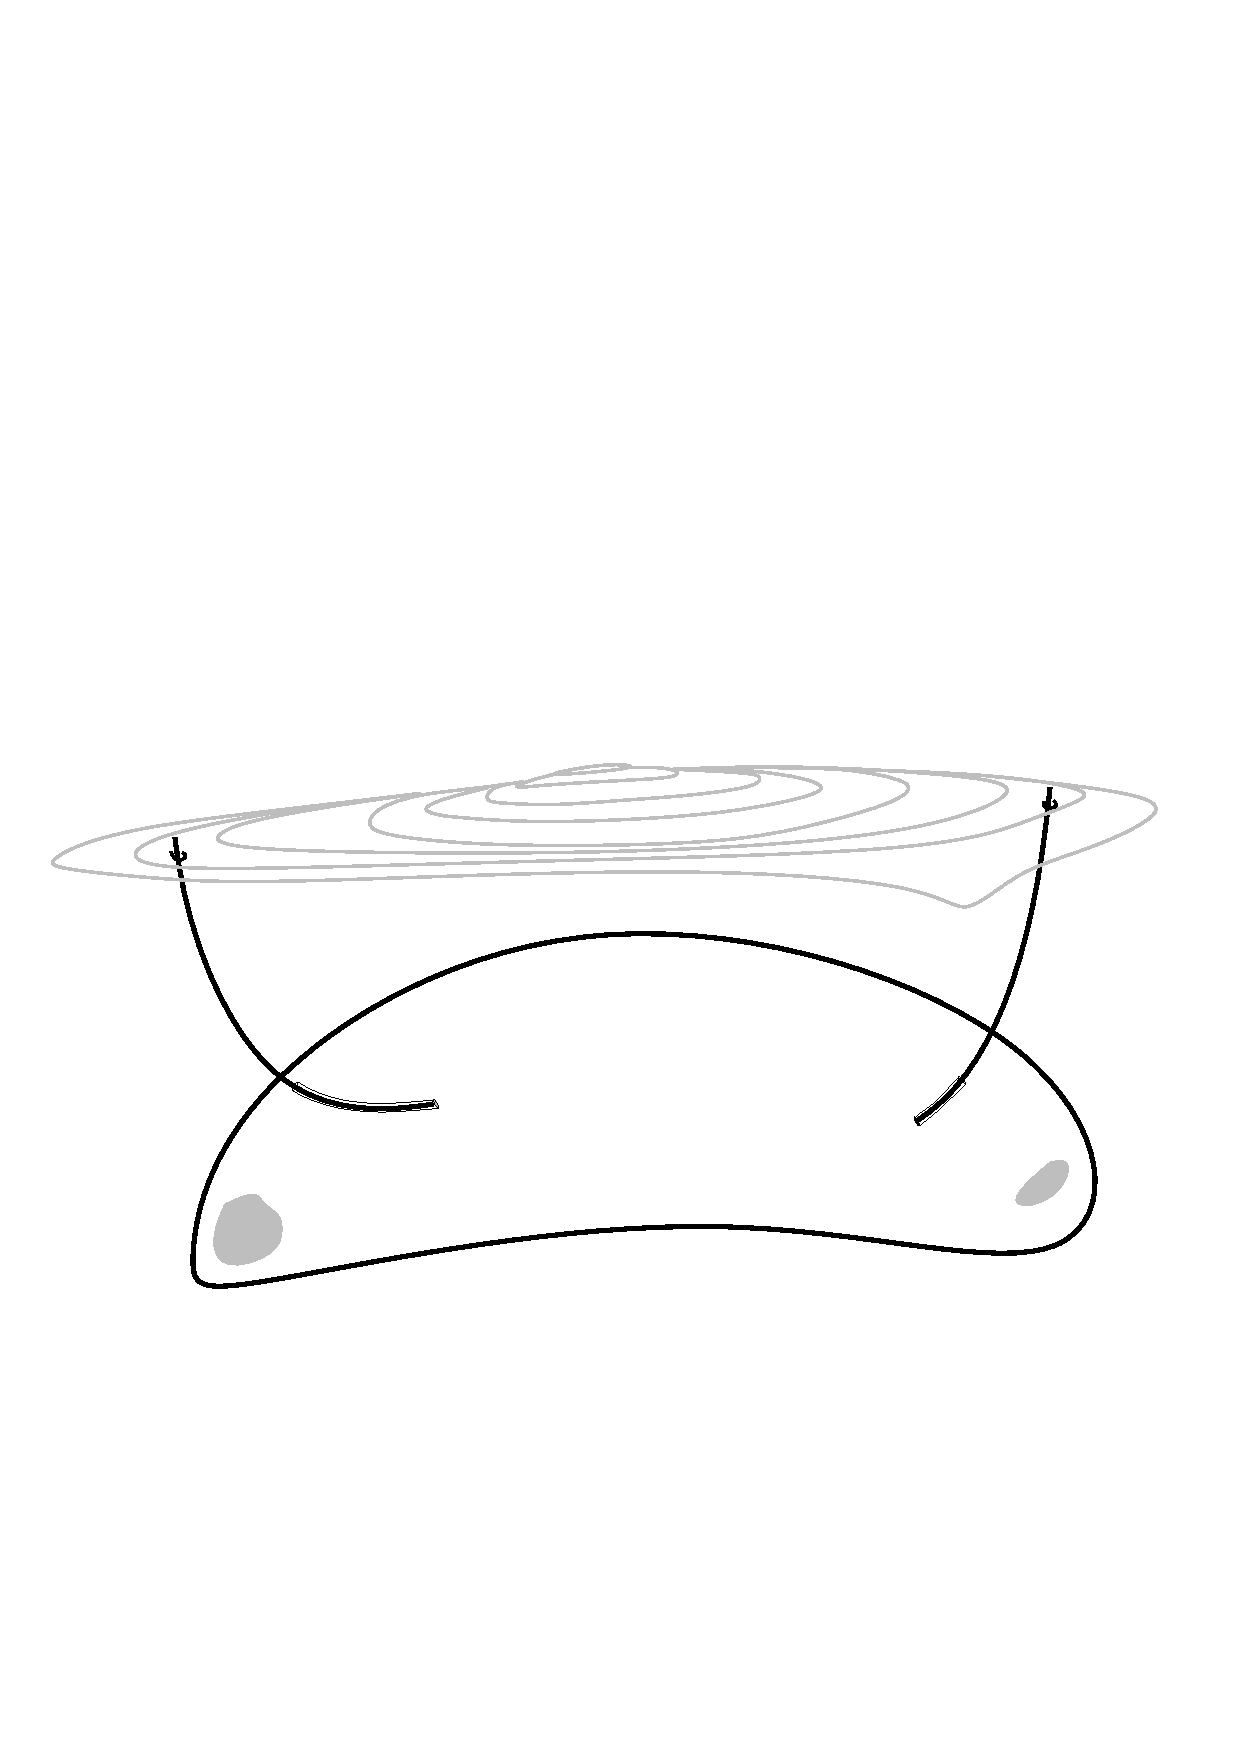
\includegraphics[scale=0.8]{Fig/yacimiento.pdf}%
	\caption[Esquemático de un yacimiento cerrado.]{Esquemático de un yacimiento cerrado. Los autores.}
	\label{fig:empanada}
\end{figure}

Además para un tiempo $t=0$ se tiene que:
\begin{align}
	P_{f}(\vec{x},0) = P^{0}_{f}(\vec{x}) \qquad \forall f \in \left\lbrace o,g,w\right\rbrace\\
	S_{f}(\vec{x},0) = S^{0}_{f}(\vec{x}) \qquad \forall f \in \left\lbrace o,g,w\right\rbrace
\end{align}
%
Es decir, existe funciones en el espacio que describen las condiciones iniciales de presión $P^{0}_{f}(\vec{x})$ y saturación $S^{0}_{f}(\vec{x})$ para los fluidos $f$ del yacimiento.

\subsection{Discretización}\label{subsec:Discretization}

Existen múltiples métodos numéricos para resolver las ecuaciones diferenciales parciales que se describen en el BOM, tales como las diferencias finitas (FDM), los volúmenes finitos (FVM), los elementos finitos (FEM), entre otros. Éstos consisten en construir un sistema de ecuaciones algebraicas para un dominio discreto, es decir, con un número finito de celdas o volúmenes de control, a partir de un dominio físico continuo, cuya solución se aproxime a la del sistema de ecuaciones diferenciales parciales original. Al proceso de construir el sistema de ecuaciones algebraico para dominios discretos se le llama discretización. En la Figura \ref{fig:EmpanadaDiscretizada} se muestra un ejemplo de un dominio discreto. Las zonas en rojo corresponden a celdas con aportes de fuentes y sumideros.\\

\begin{figure}[h]
	\centering%
	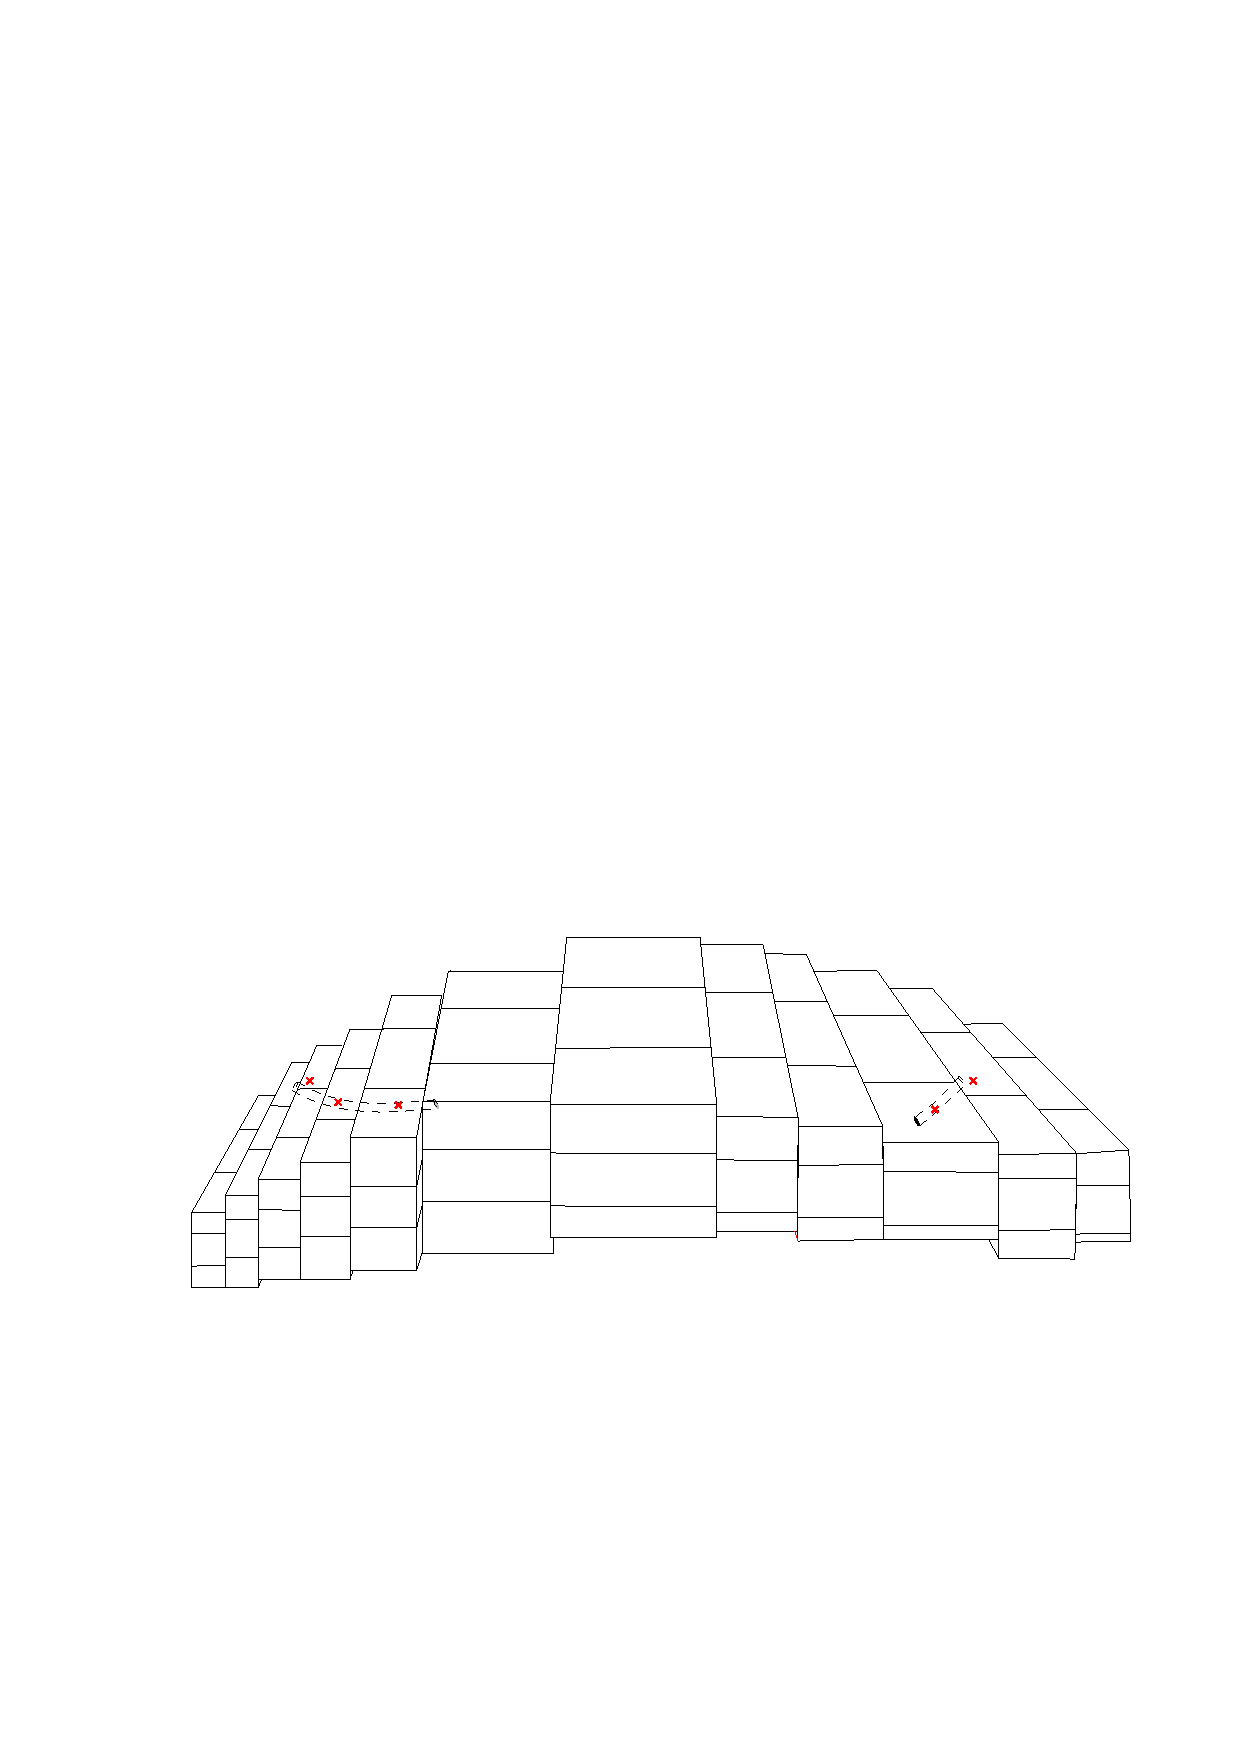
\includegraphics[scale=0.8]{Fig/yacimiento-discretizacion.pdf}%
	\caption[Ejemplo de dominio discreto.]{Ejemplo de dominio discreto. Los autores.}
	\label{fig:EmpanadaDiscretizada}
\end{figure}

Para las ecuaciones diferenciales que son dependientes del tiempo, como lo son las de BOM, se requiere, también, obtener un conjunto finito de intervalos de tiempo, para los cuales resolver las ecuaciones. Así, para un término $F(t)$ dependiente del tiempo, su integral en un intervalo $\left[t;t+\Delta t\right]$ se puede expresar, usando el teorema del valor medio como:
\begin{align}
	\int_{t}^{t+\Delta t} F(t) dt = F_{m}|\Delta t|
\end{align}
donde $F_{m} = F(t^{*})$ denota el valor promedio de la función $F$, con $t^{*} \in  \left[t;t+\Delta t\right]$. Este $t^{*}$ no se conoce, por tanto, se necesita una aproximación numérica para calcular tal valor promedio. Según la aproximación que se tome, se define el esquema de aproximación para el tiempo. Pudiendo ser:
\begin{itemize}
	\item Esquema Explícito
	\begin{align}
		\label{ec:Explicit}&F_{m} = F^{n} = F(t_{n}) = F(t)
	\end{align}
	\item Esquema Implícito
	\begin{align}
	\label{ec:Implicit}&F_{m} = F^{n+1} = F(t_{n+1}) = F(t+\Delta t)
	\end{align}
	\item Esquema Crank-Nicholson
	\begin{align}
	\label{ec:C-N}&F_{m} = \frac{F(t_{n})+F(t_{n+1})}{2} = \frac{F(t)+F(t + \Delta t)}{2}
	\end{align}
\end{itemize}
%{\color{red} Hablar de que significa la discretización y por qué es necesario, hablar de discretización espacial y discretización temporal acá. quizá sea necesario mostrar un dominio discretizado}

En esta Tesis de Maestría se elige el método de los volúmenes finitos (FVM) para las discretización espacial de las ecuaciones \ref{ec:aceite}, \ref{ec:gas} y \ref{ec:agua} y un esquema implícito (\ref{ec:Implicit}) para la discretización del tiempo, es decir, elección del tiempo al $n+1$ (futuro). El proceso de discretización se muestra en el anexo \ref{AnexoA}. Para una celda con índice $i$ con superficie $S$ como un conjunto de caras $c$, la discretización de las ecuaciones es la siguiente:
%Algebraic Equations
\begin{align}
\label{ec:aceiteDiscretizacion}&\underbrace{\frac{|\Omega_{i}|}{\Delta t}\left[ \phi_{i} \left( \frac{S_{o,i}}{B_{o,i}} + \frac{R_{v,i}S_{g,i}}{B_{g,i}}\right)\right]^{n+1}_{n}}_{\text{Acumulación - Aceite}} + 
\underbrace{\sum_{c \in S}\left[ T^{n+1}_{o,c} \Delta{\Phi_{o,c}^{n+1}} + R_{v,c}T^{n+1}_{g,c} \Delta{\Phi_{g,c}^{n+1}} \right] }_{\text{Flujo - Aceite}} - Q_{o,i}^{n+1} = 0 \\
\label{ec:gasDiscretizacion}&\underbrace{\frac{|\Omega_{i}|}{\Delta t}\left[ \phi_{i} \left( \frac{S_{g,i}}{B_{g,i}} + \frac{R_{s,i}S_{o,i}}{B_{o,i}}\right)\right]^{n+1}_{n}}_{\text{Acumulación - Gas}} + 
\underbrace{\sum_{c \in S}\left[ T^{n+1}_{g,c}\Delta{\Phi_{g,c}^{n+1} + R_{s,c}T^{n+1}_{o,c} \Delta{\Phi_{o,c}^{n+1}}} \right] }_{\text{Flujo - Gas}} - Q_{g,i}^{n+1} = 0 \\
\label{ec:aguaDiscretizacion}&\underbrace{\frac{|\Omega_{i}|}{\Delta t}\left[ \phi_{i} \left( \frac{S_{w,i}}{B_{w,i}}\right)\right]^{n+1}_{n}}_{\text{Acumulación - Agua}}
+ 
\underbrace{\sum_{c \in S}\left[ T^{n+1}_{w,c}\Delta{\Phi_{w,c}^{n+1}} \right]}_{\text{Flujo - Agua}} - Q_{w,i}^{n+1} = 0 
\end{align}
dónde:
\begin{align*}
	&\left[ \phi_{i} \left( \frac{S_{o,i}}{B_{o,i}} + \frac{R_{v,i}S_{g,i}}{B_{g,i}}\right)\right]^{n+1}_{n} = 
	\phi^{n+1}_{i} \left( \frac{S_{o,i}^{n+1}}{B_{o,i}^{n+1}} + \frac{R_{v,i}^{n+1}S_{g,i}^{n+1}}{B_{g,i}^{n+1}}\right) - \phi^{n}_{i} \left( \frac{S_{o,i}^{n}}{B_{o,i}^{n}} + \frac{R_{v,i}^{n}S_{g,i}^{n}}{B_{g,i}^{n}}\right),\\
	&\left[ \phi_{i} \left( \frac{S_{g,i}}{B_{g,i}} + \frac{R_{s,i}S_{o,i}}{B_{o,i}}\right)\right]^{n+1}_{n} = 
	\phi^{n+1}_{i} \left( \frac{S_{g,i}^{n+1}}{B_{g,i}^{n+1}} + \frac{R_{s,i}^{n+1}S_{o,i}^{n+1}}{B_{o,i}^{n+1}}\right) - \phi^{n}_{i} \left( \frac{S_{g,i}^{n}}{B_{g,i}^{n}} + \frac{R_{s,i}^{n}S_{o,i}^{n}}{B_{o,i}^{n}}\right),\\
	&\left[ \phi_{i} \left( \frac{S_{w,i}}{B_{w,i}}\right)\right]^{n+1}_{n} = 
	\phi^{n+1}_{i} \left( \frac{S_{w,i}^{n+1}}{B_{w,i}^{n+1}}\right) - \phi^{n}_{i} \left( \frac{S_{w,i}^{n}}{B_{w,i}^{n}}\right)
\end{align*}
El término $T_{f,c}$ en la Ecuación \ref{ec:Transmissibity} corresponde a la transmisividad en una cara $c$ que conecta una celda $i$ con otra celda $j$.
\begin{align}
	\label{ec:Transmissibity}& T_{f,c} = \left(\frac{2}{(\Delta l_{i}/A_{c}K_{l,i})+(\Delta l_{j}/A_{c}K_{l,j})}\right)\frac{k_{rf,c}}{\mu_{f,c}B_{f,c}}
\end{align}
\subsection{Modelado de Pozos}
%
Los pozos son el principal objeto de estudio de la simulación de yacimientos de petróleo, debido a que en ellos, se concentra el propósito de cualquier operación de campo. Éstos tienen dos tipos, inyector o productor, y se forman por un conjunto de bloques perforados en los que existe un flujo radial \citep{peaceman1983interpretation}. \cite{peaceman1983interpretation} describe el flujo en pozos con varias capas de perforados como se muestra en la Ecuación \ref{ec:peaceman}. En la Figura \ref{fig:mulperfwell} se ilustra un pozo vertical con múltiples perforados.

\begin{figure}[h]
	\centering%
	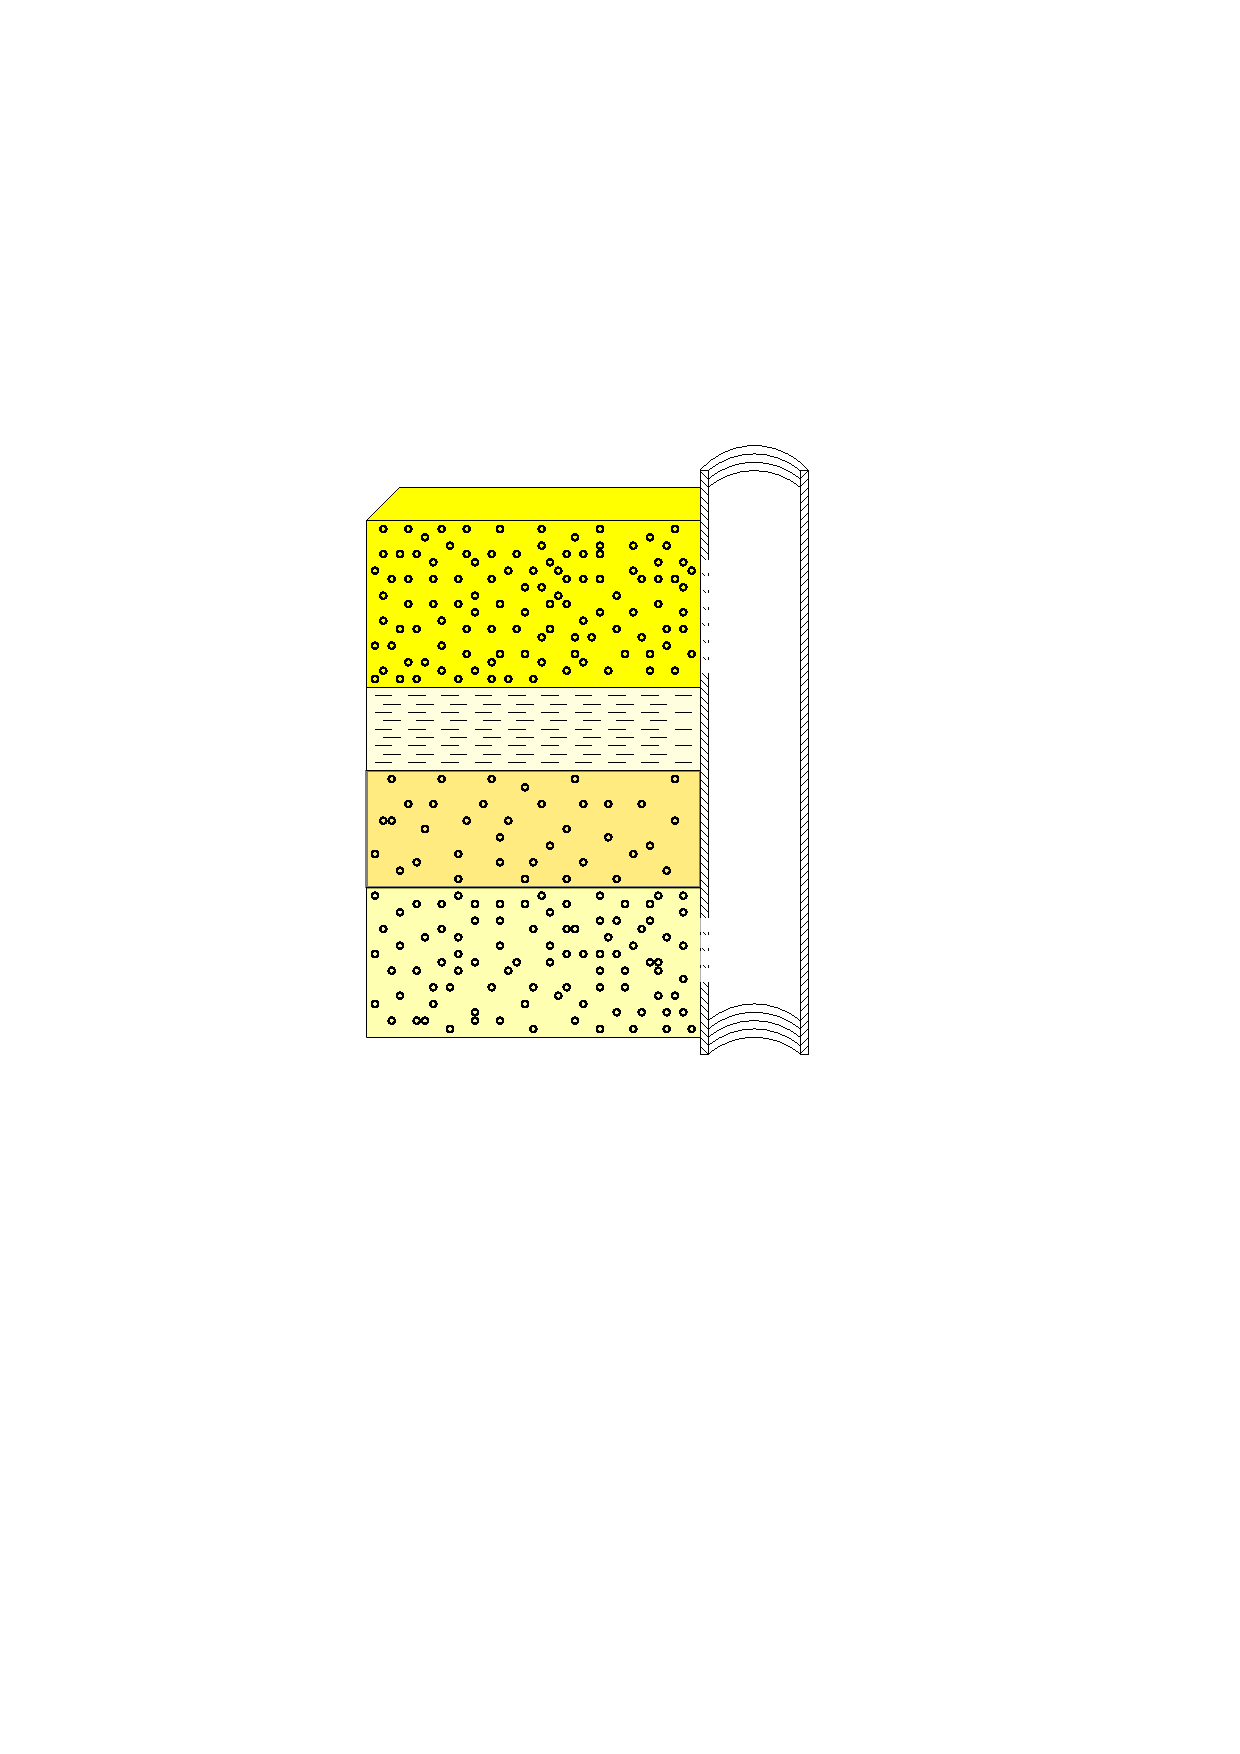
\includegraphics[scale=0.8]{Fig/pozo_multi_perf.pdf}%
	\caption[Esquemático de pozo multiperforado.]{Esquemático de pozo multiperforado. Elaboración a partir de \cite{chen2007reservoir}.} \label{fig:mulperfwell}
\end{figure}
\begin{footnotesize}
	\begin{align}
	\label{ec:peaceman}&q^{(v)}_{f, sc} = \sum_{m=1}^{M^{(v)}_{w}}\frac{2\pi k_{rf,m} \rho_{f,m} \sqrt{k_{xx,m}k_{yy,m}}h_{z,m}}{B_{f,m}\mu_{f,m}\left(\ln \left(r_{e,m}/r_{w}\right) +s_{m}\right)}\left(p_{bh}^{(v)}-p_{p,m}-\gamma_{f,bh}\left(z_{bh}^{(v)}-z_{m}\right)\right)\delta\left(x-x_{m}^{(v)}\right)
	\end{align}
\end{footnotesize}
Donde $v$ corresponde al índice del pozo, $M_{w}$ a la cantidad de perforados y $m$ al índice de cada perforado, que debe coincidir con el de una celda; y $P_{p}$ es la presión del perforado.\\

Además, los pozos se controlan por condiciones operativas, que permiten mantener un régimen conocido de presión o caudal, tanto en inyección como producción. Las condiciones operativas también dependen del tipo del pozo. Sin embargo, en esta Tesis de Maestría sólo se consideran dos tipos de condición operativa, presión y caudal a condiciones estándar. Donde, para un pozo productor es caudal de líquido, es decir, caudal de aceite más el de agua; y para un pozo inyector es el caudal del fluido de inyección. Luego para el caudal de un pozo productor:
\begin{align}
	q^{v}_{prod,sc} = q^{v}_{o,sc} + q^{v}_{w,sc}
\end{align}
Donde $q^{v}_{f,sc}$ para $f \in \left\lbrace o,w \right\rbrace$ se calcula usando la Ecuación \ref{ec:peaceman}.\\

Para un pozo inyector, se necesita calcular la movilidad del fluido de inyección, sumando las movilidades de los fluidos que debe desplazar en el mismo, porque el influjo está dominado por los fluidos que se desplazan. Por tanto, el caudal de inyección es:

\begin{scriptsize}
	\begin{align}
	\label{ec:peacemaniny}&q^{(v)}_{iny, sc} = \sum_{m=1}^{M^{(v)}_{w}}\left(\sum_{f \in F}\frac{k_{rf,m}}{\mu_{f,m}}\right)\frac{2\pi \rho_{iny,m} \sqrt{k_{xx,m}k_{yy,m}}h_{z,m}}{B_{iny,m}\left(\ln \left(r_{e,m}/r_{w}\right) +s_{m}\right)}\left(p_{bh}^{(v)}-p_{p,m}-\gamma_{iny,bh}\left(z_{bh}^{(v)}-z_{m}\right)\right)\delta\left(x-x_{m}^{(v)}\right)
	\end{align}
\end{scriptsize}

Donde $iny$ corresponde al fluido de inyección y $f \in F:\left\lbrace o,g,w,... \right\rbrace$ a los fluidos en el dominio físico.
%{\color{red} No he hablado de condiciones operativas}

\subsection{Método de Newton-Raphson}\label{subsec:N-R}
%
El sistema de ecuaciones algebraicas que se forman por \ref{ec:aceiteDiscretizacion}, \ref{ec:gasDiscretizacion} y \ref{ec:aguaDiscretizacion} es no lineal, por lo tanto, se aplica el método del Newton-Raphson el cuál se usa para encontrar las raíces de una ecuación no lineal aproximando su derivada, como se ilustra en la Figura \ref{fig:NewtonR}.
El método de Newton-Raphson se presenta en la Ecuación \ref{ec:Newton-R} hasta la Ecuación \ref{ec:Derivative}.

\begin{figure}[h]
	\centering%
	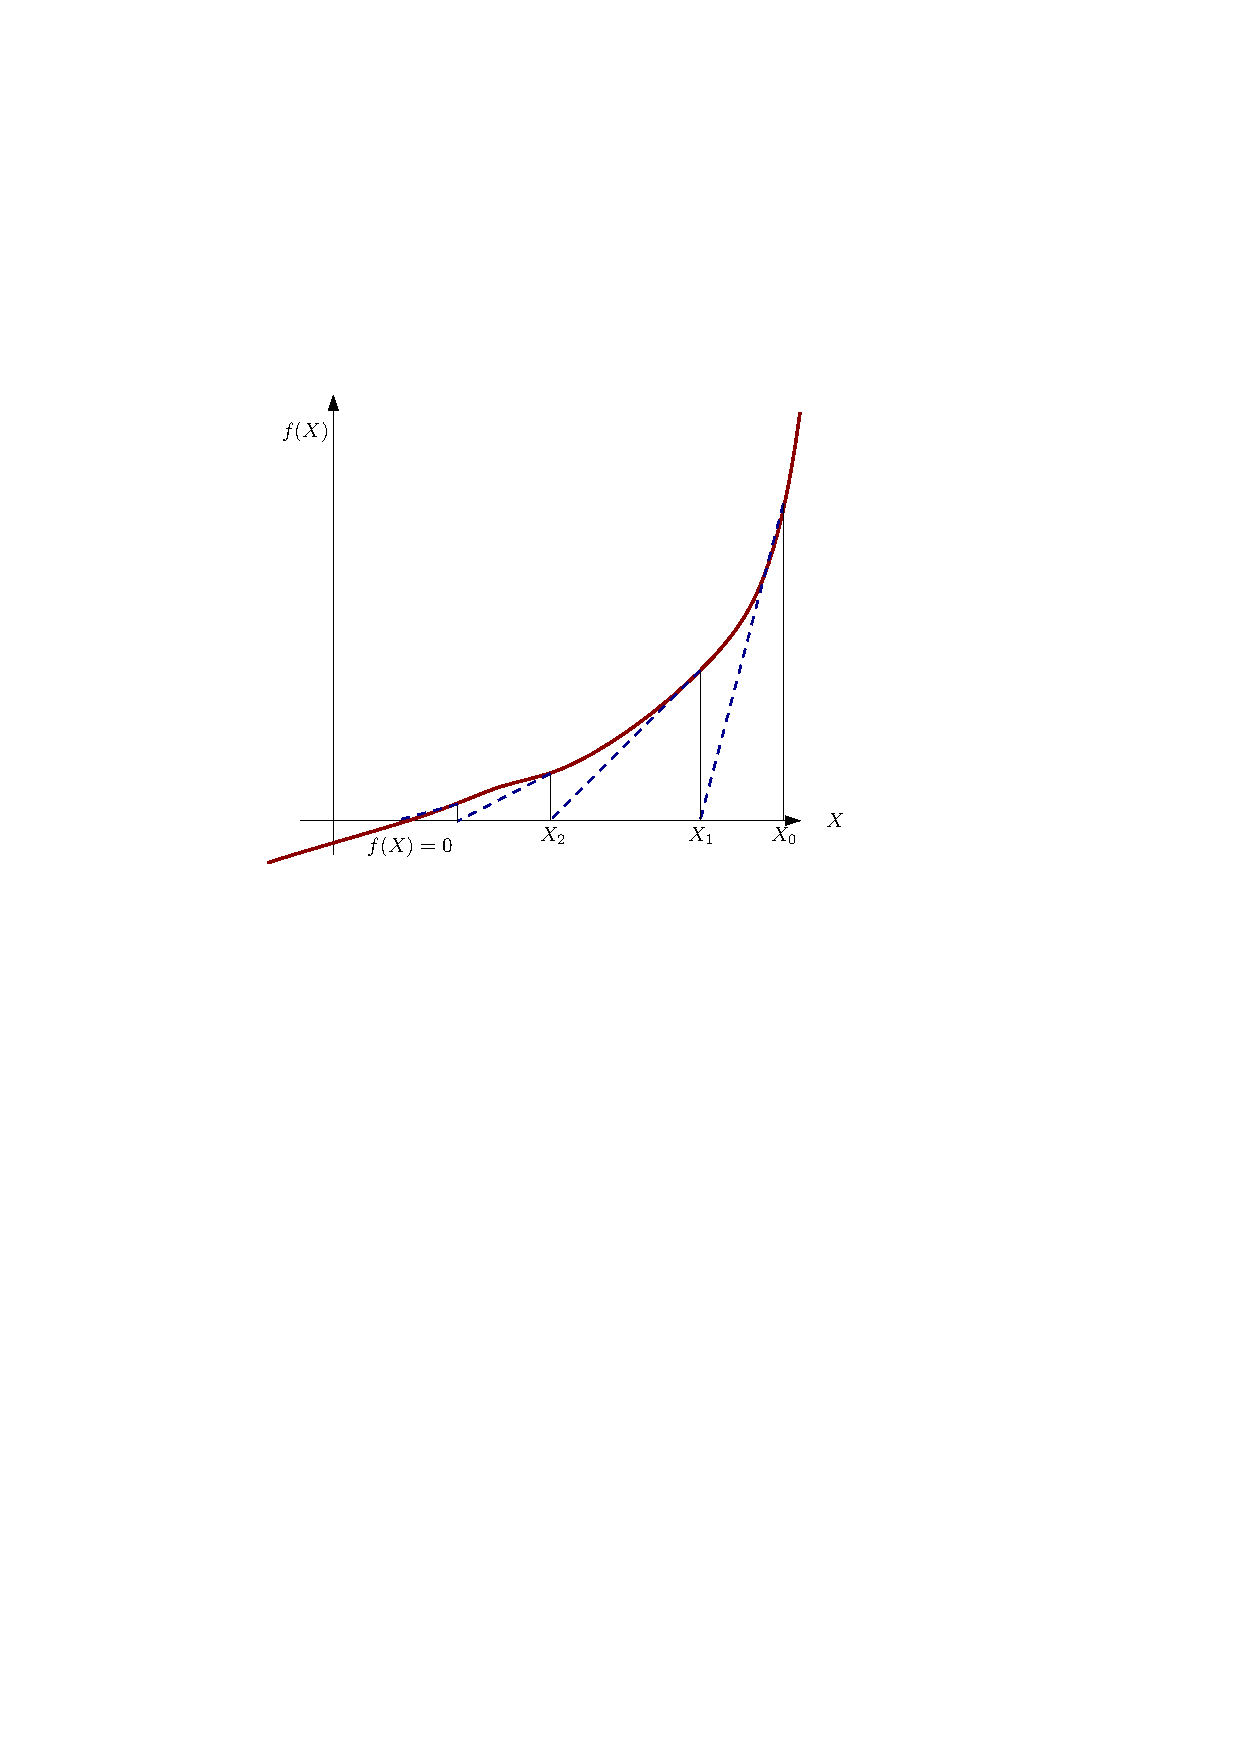
\includegraphics[scale=0.8]{Fig/NewtonR.pdf}%
	\caption[Aproximación a la derivada de una función.]{Aproximación a la derivada de una función. Elaboración a partir de \cite{atkinson2008introduction}.} \label{fig:NewtonR}
\end{figure}
\begin{align}
\label{ec:Newton-R}&A \cdot {\Delta \vec{x}} = \vec{b} \Leftrightarrow J^{k}_{i,j} \cdot {\Delta \vec{x}} = -\vec{R^{k}_{i}}\\
&\Delta \vec{x} = \vec{x}^{k+1} - \vec{x}^{k} = \left(\Delta P_o, \Delta S_g, \Delta S_w \right)^T\\
&-\vec{R^k_i} = \left(\Delta R^k_{P_o,i}, \Delta R^k_{S_g,i}, \Delta R^k_{S_w,i} \right)^T\\
&J^k_{i,j}=\frac{\partial R^k_i}{\partial x^k_j}\\	
\label{ec:Derivative}&\frac{\partial R^k}{\partial x^k} \approx \frac{R\left(x^k + \xi \right) - R\left(x^k \right)}{\xi}
\end{align}

\section{Procesos de Recobro Mejorado}\label{sec:EOR}
El recobro mejorado químicamente se enmarca en los procesos de recobro mejorado (EOR), se considera como una técnica eficiente de recuperación de petróleo para producir el aceite residual atrapado en yacimiento o que se puede extraer de manera económica por métodos convencionales. Los métodos EOR, se basan en la inyección de productos químicos para impulsar la recuperación de petróleo, cambiando interacciones de los fluidos con el yacimiento \citep{gbadamosi2019overview}.\\

Durante la recuperación de petróleo, el desplazamiento general del fluido se debe a una combinación de barrido macroscópico (barrido volumétrico) y de una eficiencia de desplazamiento microscópico (escala de poro). \cite{olajire2014review} y \cite{samanta2012comparative}, proponen que ambos factores se afectan por propiedades objetivo de los fluidos y de la roca, que se cambian debido a interacción con los químicos que se inyectan o producen en un yacimiento. En la Figura \ref{fig:diagrama_eor} se ilustran los procesos de recobro mejorado (EOR) existentes, en esta Tesis de Maestría se representan los procesos EOR que se basan en la inyección de químicos, tal como se muestra en el recuadro rojo.

\begin{figure}
	\centering
	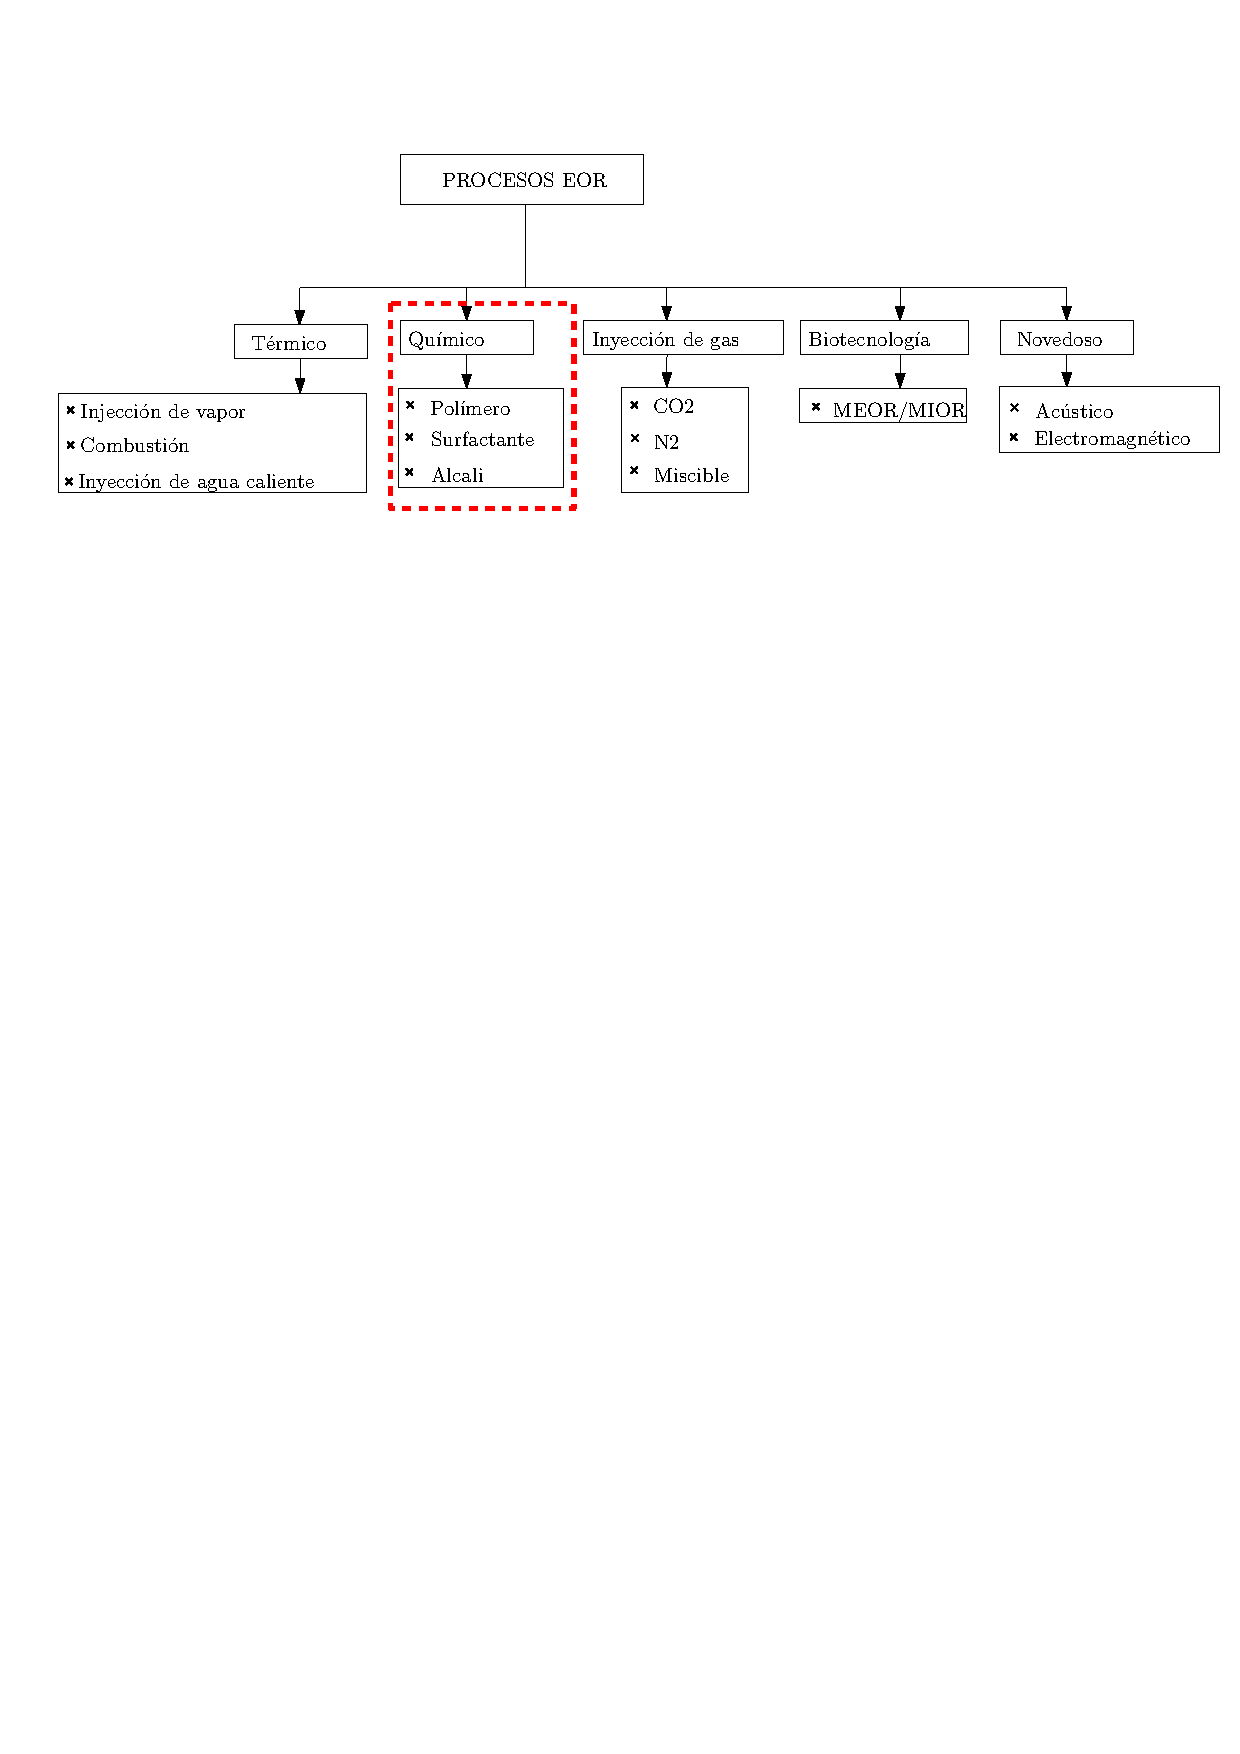
\includegraphics[width=0.9\textwidth]{Fig/diagramaEOR.pdf}
	\caption[Diagrama de división de procesos EOR.]{Diagrama de división de procesos EOR. Elaboración a partir de \cite{gogoi2013carbon}.}
	\label{fig:diagrama_eor}
\end{figure}{}

%\subsection{Modelado del Químico}\label{subsec:Chemical}
%
%
%
%\begin{equation}
%\begin{split}
%B_{j}T_{j}^{n+1}y_{i,j}^{n+1}(\Delta \Phi^{n+1}_{j}) + q_{i,j}^{n+1} + \sum_{k=1, k\neq j}^{n_{p}}(\dot{m}^{n+1}_{j \rightarrow k})- \frac{V}{\Delta t}\left[ N_{i,j}^{n+1}-N_{i,j}^{n} \right]=0\\
%para\; i = 1,..., n_{c}\\
%para\; j = 1,..., n_{p}
%\end{split}{}    
%\label{eqholi}
%\end{equation}{}
%\section{Procesos de Recobro Mejorado}

\section{Esquemas Preconceptuales}\label{sec:EP}

Los Esquemas Preconceptuales (EP) son representaciones intermedias entre el lenguaje natural y un esquema conceptual o un lenguaje formal. Estos esquemas contienen todo el dominio de aplicación de un interesado y, por tanto, sirven para establecer un punto común de entendimiento entre un interesado y un analista de software \citep{zapata2007phd}. Los EP se desarrollan con la idea de mantener la coherencia y consistencia entre el discurso del interesado y el software que se desarrolla. 

\subsection{Elementos del Esquema Preconceptual}\label{subsec:ElementsEP}
\cite{zapata2012unc} define los elementos del EP tal como se observa en la Figura \ref{fig:InitialPS} para la representación del dominio del interesado. Estos elementos se dividen en cuatro categorías: nodos, relaciones, enlaces, y aglutinadores.\\

\begin{figure}[h]
	\centering%
	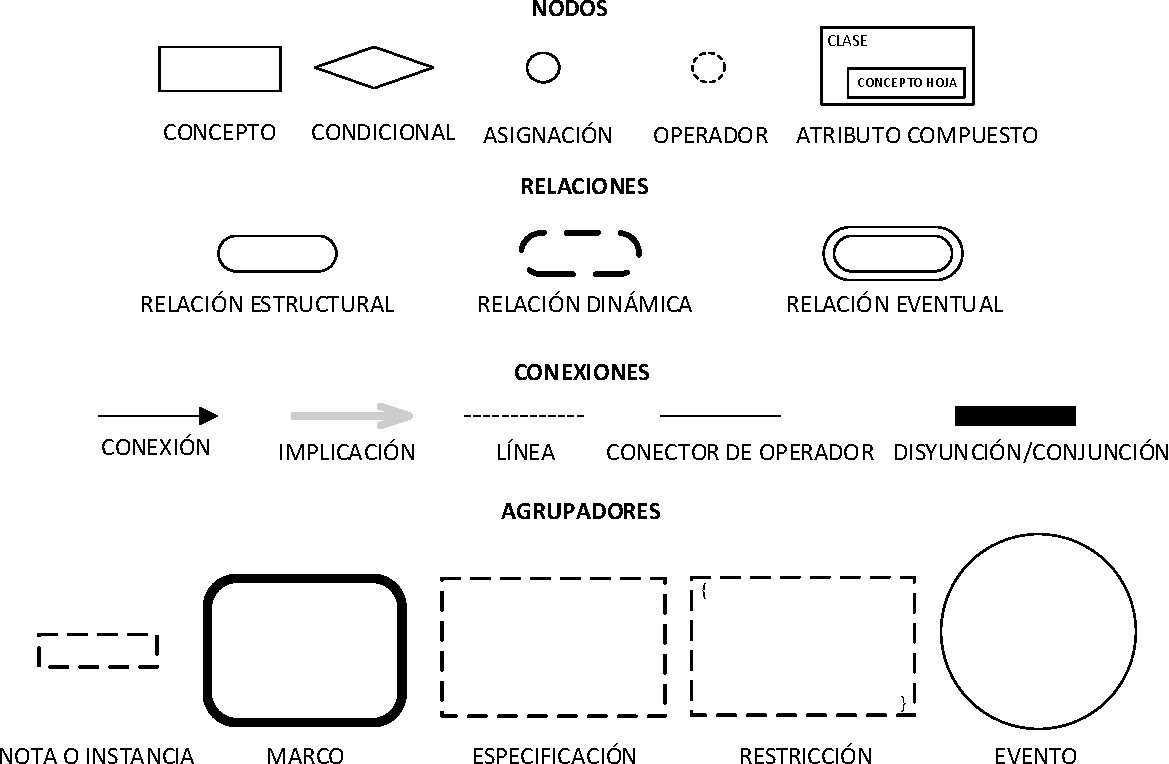
\includegraphics[scale=0.51]{Fig/ElementosDelEP.pdf}%
	\caption[Elementos del EP.]{Elementos del EP. \citep{zapata2012unc}.} \label{fig:InitialPS}
\end{figure}

\subsubsection{Nodos}
\begin{itemize}
	\item \textbf{Concepto}:
	sustantivo o sintagma nominal que representa un actor u objeto dentro del dominio del interesado. Se subclasifican en conceptos clase y conceptos hoja, según su jerarquía \citep{zapata2007phd,zapata2012unc}. %En la figura \ref{fig:PS_Concept} se muestra la representación. Un ejemplo de su uso se presenta en la figura \ref{fig:ej_concept}.
	
	\item \textbf{Condicional}: condición para ejecutar una relación dinámica o una especificación a partir de una expresión lógica formada por conceptos o variables, operadores, y valores o parámetros \citep{zapata2007phd,zapata2012unc}. %como se muestra en la figura \ref{fig:}
	
	\item \textbf{Operador}: símbolo lógico o matemático que sirve para formar expresiones a evaluar \citep{zapata2012unc}.
	
	\item \textbf{Asignación}: Sirve para asignar el valor que resulta de una expresión matemática o lógica \citep{zapata2012unc}.
	
	\item \textbf{Concepto Clase}: Sirve para representar el acceso a un concepto hoja o atributo desde su concepto contenedor \citep{zapata2007phd}.
\end{itemize}

\subsubsection{Relaciones}
\begin{itemize}
	\item \textbf{Relación Estructural}: Relación permanente entre dos conceptos. Se asocia con los verbos ``ser'' o ``tener'', y que significan generalización o agregación, respectivamente \citep{zapata2007phd,zapata2012unc}.
	\item \textbf{Relación Dinámica}: Se asocia con verbos que denotan acción u operaciones que modifican el dominio de estudio; permite establecer relaciones transitorias entre el concepto ejecutor de la acción y el concepto objeto de dicha acción \citep{zapata2007phd,zapata2012unc}.
	\item \textbf{Relación Eventual}: Se relaciona con un verbo que denota ocurrencia, el cuál no se asocia a un concepto ejecutor. \citep{zapata2012unc,norena2018Ling}.
\end{itemize}

\subsubsection{Enlaces}
\begin{itemize}
	\item \textbf{Conexión}: Es una flecha unidireccional que sirve para conectar conceptos con relaciones dinámicas o estructurales \citep{zapata2007phd,zapata2012unc}.
	\item \textbf{Implicación}: Es una línea continua y dirigida que sirve para indicar una relación causa-efecto u orden entre relaciones dinámicas, condicionales o eventos. \citep{zapata2007phd,zapata2012unc}. 
	\item \textbf{Concepto-Nota}: Sirve para conectar un concepto a una nota o instancia \citep{zapata2007phd,zapata2012unc}.
	\item \textbf{Conector de Operador}: Sirve para conectar un valor, concepto, atributo compuesto u otros operadores, a un operador \citep{zapata2012unc}. 
	\item \textbf{Conjunción/Disyunción}: Sirve para agrupar o bifurcar implicaciones, estableciendo una causalidad conjunta o múltiples efectos \citep{zapata2007phd,zapata2012unc}. 
\end{itemize}

\subsubsection{Aglutinadores}
\begin{itemize}
	\item \textbf{Nota o Instancia}: Sirve para limitar los valores para un concepto a un conjunto predefinido \citep{zapata2007phd,zapata2012unc}.
	\item \textbf{Especificación}: Sirve para agrupar un conjunto de operaciones que describen una relación dinámica o eventual \citep{zapata2012unc}.
	\item \textbf{Marco}: Sirve para asociar múltiples relaciones dinámicas a una responsabilidad o para agrupar conceptos \citep{zapata2012unc}.
	\item \textbf{Restricción}: Sirve para establecer una condición sobre una especificación de operaciones \citep{zapata2012unc}. Adicionalmente, se usa para establecer ciclos sobre conceptos o condiciones \citep{JChaverra}.
	\item \textbf{Evento}: Es una ocurrencia que habilita cambios de estado en los procesos  \citep{zapata2013Eventos}.
\end{itemize}

\subsection{Esquemas Preconceptuales en el contexto del software científico}\label{subsec:EPScientific}

\cite{JCalle} y \cite{norena2018det} descubren la capacidad del EP para representar aplicaciones en el contexto del software científico. Para ello, definen elementos adicionales que permiten modelar dominios de mayor complejidad. En esta Tesis de Maestría se usan las condiciones iniciales, conceptos tipo arreglo, parámetros, variables, vectores, operadores predefinidos, operador ``\textit{push}'', operador ``\textit{type}'',  y funciones que define el analista. En la Figura \ref{fig:NewElements} se representan los elementos previamente mencionados. A continuación, se explican los elementos adicionales que se usan en el desarrollo de esta Tesis de Maestría.

\begin{figure}[h]
	\centering%
	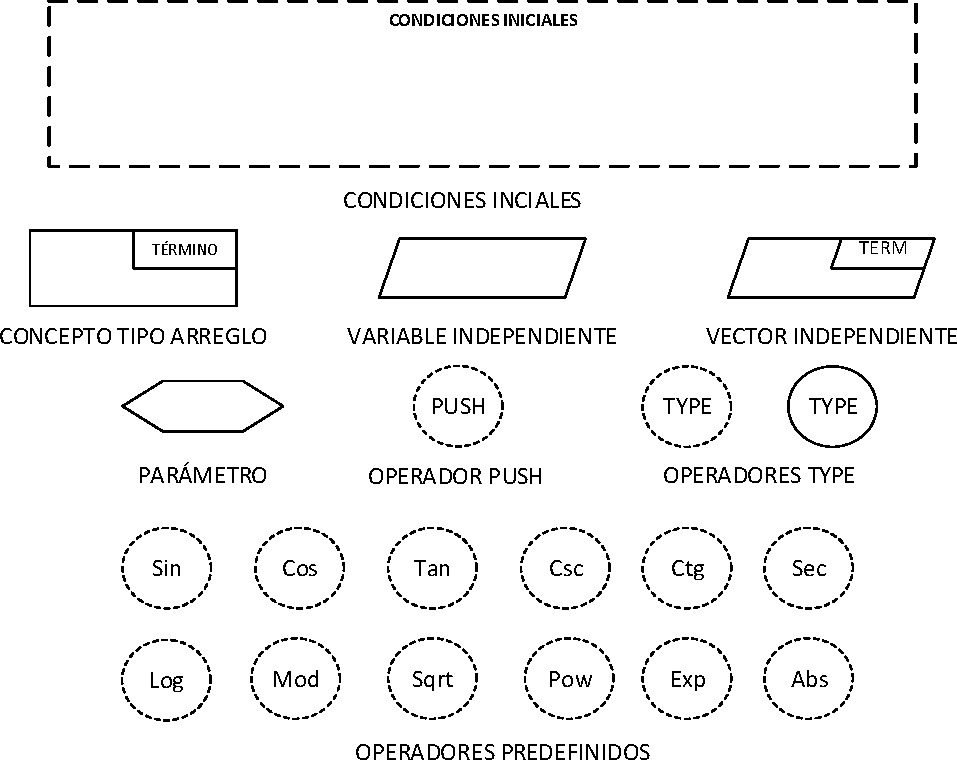
\includegraphics[width=0.9\linewidth]{Fig/NuevosElementosDelEP.pdf}%
	\caption[Elementos para la representación de Software Científico.]{Elementos para la representación de Software Científico. \citep{JCalle,norena2018det}.} \label{fig:NewElements}
\end{figure}

\subsubsection{Condiciones Iniciales}
Las condiciones iniciales son especificaciones, de variables y parámetros globales, que se conoce desde el inicio de la simulación \citep{norena2018det}. Un ejemplo de uso se presenta en la Figura \ref{fig:EjInitialConditions}.

\begin{figure}[h]
	\centering%
	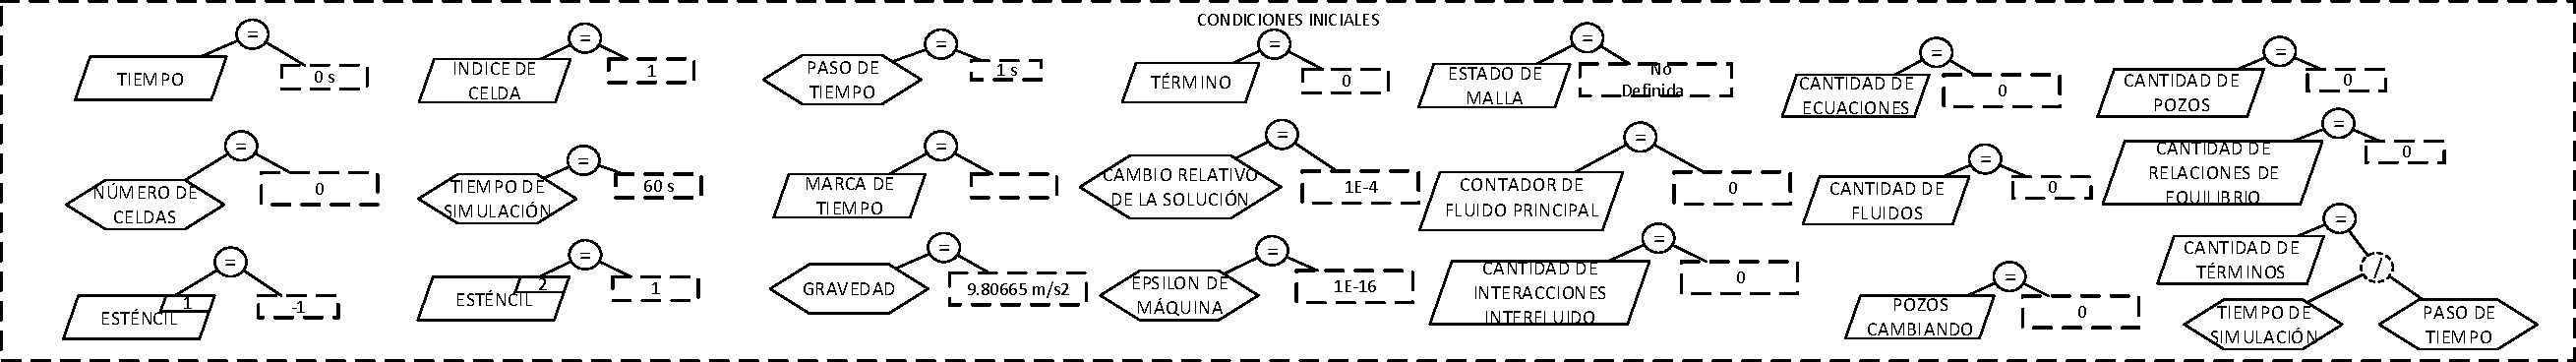
\includegraphics[width=0.9\linewidth]{Fig/EjInitialConditions.pdf}%
	\caption[Ejemplo de Condiciones Iniciales.]{Ejemplo de Condiciones Iniciales. Los autores.} \label{fig:EjInitialConditions}
\end{figure}

\subsubsection{Concepto tipo arreglo}
Los conceptos tipo arreglo permiten almacenar de manera permanente múltiples valores, y a su vez, iterar sobre ellos \citep{JCalle}. En esta Tesis de Maestría se usan conceptos tipo arreglos multidimensionales. En la Figura \ref{fig:EjArrConcept} se expone un ejemplo de su uso.

\begin{figure}[h]
	\centering%
	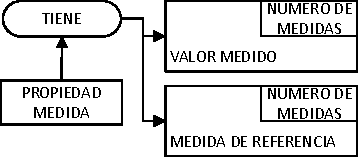
\includegraphics[scale=1]{Fig/EjArrConcepts.pdf}%
	\caption[Ejemplo de Conceptos tipo arreglo.]{Ejemplo de Conceptos tipo arreglo. Los autores.} \label{fig:EjArrConcept}
\end{figure}

\subsubsection{Parámetro}
Los parámetros se usan para almacenar constantes o definir entradas en la especificación de relaciones dinámicas, especificaciones de tipo marco y funciones, que reciben múltiples argumentos o parámetros \citep{JCalle, norena2018det}. Se expone un ejemplo de uso en la Figura \ref{fig:EjParameter}.\\

\begin{figure}[h]
	\centering%
	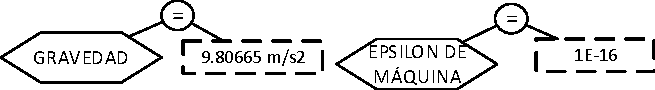
\includegraphics[width=0.5\linewidth]{Fig/EjParametro.pdf}%
	\caption[Ejemplo de parámetros.]{Ejemplo de parámetros. Los autores.} \label{fig:EjParameter}
\end{figure}

\subsubsection{Variable Independiente}
Las variables independientes permiten almacenar valores durante la ejecución de una especificación sin estar acopladas a un concepto. Si se definen en las condiciones iniciales, se pueden usan de manera global durante toda la simulación \citep{norena2018det}. En la Figura \ref{fig:EjInitialConditions} se pueden ver ejemplos de variables independientes.\\

\subsubsection{Vector independiente}
Los vectores independientes cumplen la misma tarea y propiedades de las variables independientes, pero permiten almacenar más de un valor \citep{norena2018det}. Un ejemplo de vector independiente se presenta en la Figura \ref{fig:EjVector}.

\begin{figure}[h]
	\centering%
	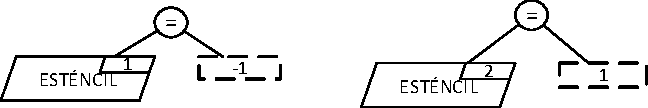
\includegraphics[width=0.5\linewidth]{Fig/EjVectorIndependiente.pdf}%
	\caption[Ejemplo de vector independiente.]{Ejemplo de vector independiente. Los autores.} \label{fig:EjVector}
\end{figure}

\subsubsection{Operadores Predefinidos}
Son funciones algebraicas y trigonométricas predefinidas que se pueden usar como operadores en el EP \citep{JCalle}.

\subsubsection[Operador \emph{Push}]{Operador {\normalfont \bfseries \itshape Push}}
El operador \textit{Push} sirve para insertar, valores, conceptos o parámetros dentro de un concepto tipo arreglo, el elemento que se inserta queda en la última posición del arreglo  \citep{JCalle}.
\subsubsection[Operador \emph{Type}]{Operador {\normalfont \bfseries \itshape Type}}
El operador \textit{Type} tiene dos versiones: una como operador de asignación y otra como operador de información. En el caso de la asignación, sirve para otorgarle el tipo de una subclase a un concepto. Mientras que en el de información, permite consultar si el tipo del concepto corresponde con el tipo de una subclase definida \citep{JCalle}.
\subsubsection{Funciones que define el analista}
Las funciones que define el analista son especificaciones reutilizables en el EP a modo de un operador personalizado cuyo nombre define el analista. Estas funciones llevan en su especificación un concepto ``\textit{return}'' que corresponde al valor que devuelve la función cuando se usa como operador \citep{JCalle}. En la figura \ref{fig:Potencial} se presenta un ejemplo de definición y uso de una función que define el analista.

\begin{figure}[h]
	\centering%
	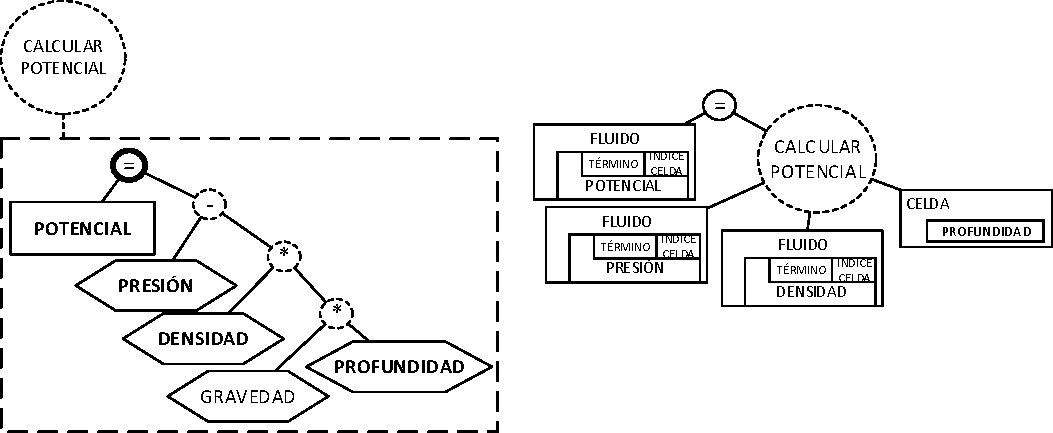
\includegraphics[scale=0.8]{Fig/EjFuncion.pdf}%
	\caption[Ejemplo de función, cálculo del potencial.]{Ejemplo de función, cálculo del potencial. Los autores.} \label{fig:Potencial}
\end{figure}

\section{Modelo Ejecutable}\label{sec:Executable}
Un modelo ejecutable es una abstracción que permite describir y definir la conceptualización y comportamiento de un dominio real o hipotético de estudio. Además, cuentan con semánticas que permiten definir acciones \citep{ExecutableUML}. El EP se enmarca dentro de esta definición, puesto que los EP ejecutables tienen elementos que permiten representar acciones que se procesan internamente en el modelo \citep{JChaverra}. 